\documentclass[a4paper,10pt]{article}

% IMPORTS
\usepackage{amsfonts}
\usepackage{amsmath}
\usepackage{amssymb}
\usepackage{graphicx}
\usepackage{titlesec}
\usepackage{wrapfig}
\usepackage[ngerman]{babel}
\usepackage[utf8x]{inputenc}
\usepackage{pdfpages}
\usepackage{placeins}
\usepackage{color}
\usepackage{eurosym}
\usepackage{xargs}
\usepackage{xcolor}
\usepackage{subcaption}
\usepackage{hyperref}
\usepackage[margin=2cm]{geometry}
\usepackage[colorinlistoftodos,prependcaption,textsize=tiny]{todonotes}

% CONFIG
\clubpenalty = 9000
\widowpenalty = 9000
\displaywidowpenalty = 9000
\titlespacing\subsection{0pt}{14pt plus 4pt minus 2pt}{2pt plus 2pt minus 1pt}
\titlespacing\subsection{0pt}{10pt plus 4pt minus 2pt}{2pt plus 2pt minus 1pt}
\setlength{\parindent}{0pt}
\setcounter{tocdepth}{2}

% -----------------------------------------------------------------------------
\begin{document}

\begin{titlepage}
	\begin{center}
		\huge Notizen zum \\
		\Huge \textbf{Basiskurs Mathematik} \\
		\huge bei Prof. Kreuzer im WS 16/17 \\
		\normalsize

		\vspace{1cm}
		\begin{tabular}[b]{l|l}
			\textbf{author} & Niko Fink \texttt{<finksim@fim.uni-passau.de>} \\
							& Maximilian Reif \texttt{<reifmaxi@fim.uni-passau.de>} \\
							& Lars Friedrich \texttt{<friedril@fim.uni-passau.de>} \\
			\textbf{last change} & \today
		\end{tabular}

		\vspace{1cm}
		\tableofcontents
	\end{center}
\end{titlepage}

\section{Algebra}

\subsection{Formeln}
\begin{align}
(a+b)^2 &= (a^2 + 2ab + b^2) \tag{1. binomische Formel} \\
(a-b)^2 &= (a^2 - 2ab + b^2) \tag{2. binomische Formel} \\
(a+b)(a-b) &= (a^2 - b^2) \tag{3. binomische Formel} \\
1-a^{n+1} &= (1 + a + a^2 + a^3 + \cdots + a^n) * (1-a) \tag{Teleskopsumme} \\
1+a^{n}   &= (1 - a + a^2 - a^3 + \cdots + a^{n-3} - a^{n-2} + a^{n-1}) * (1+a) \text{ falls n ungerade} \tag{Teleskopsumme2} \\
a^n - b^n &= (a-b) * (a^{n-1} + a^{n-2} b + a^{n-3} b^2 + \cdots + ab^{n-2} +b^{n-1}) \\
a^n + b^n &= (a+b) * (a^{n-1} - a^{n-2} b + a^{n-3} b^2 - \cdots b^{n-1}) \\
a^3 + b^3 &= (a+b) * (a^2 - ab + b^2)
\end{align}

\subsection{Lösen von quadratischen Gleichungen}
Seinen $a,b,c \in \mathbb{R} \text{ oder } \mathbb{C} \text{ mit } a \neq 0$, dann heißt $ax^2 + bx +c = 0$ eine quadratische Gleichung mit einer Unbestimmten.
\begin{enumerate}
\item Wegen $a \neq 0$ kann man durch $a$ teilen und erhält
	\[x^2 + px + q = 0 \text{ mit } p=\frac{b}{a}, q=\frac{c}{a}\]
\item Quadratische Ergänzung
	\[\overbrace{\left( x + \frac{p}{2} \right)^2}^{=x^2 + 2*\frac{p}{2}*x + \frac{p^2}{4}} - \frac{p^2}{4} + q = 0\]
\item Wurzel ziehen
	\[\left( x + \frac{p}{2} \right)^2 = \frac{p^2}{4} - q = \frac{p^2 - 4q}{4}\]
	Ist $p^2-4q < 0$ so gibt es in $\mathbb{R}$ keine Lösung, ansonsten ist $x+\frac{p}{2} = \pm \frac{1}{2} \sqrt{p^2-4q}$
\end{enumerate}
\subsubsection*{Mitternachtsformel}
\[x_1,x_2 = \frac{-b \pm \sqrt{b^2-4ac}}{2a}\]

\subsection{Satz von Vietá}
Seien $x_1, x_2$ die Lösungen einer quadratischen Gleichung $x^2+px+q=0$, dann gilt $x_1+x_2=-p$ und $x_1*x_2=q$.
Finde dann über die Teiler von $q$ die Werte von $x_1, x_2$ durch ausprobieren.

\subsection{Dreiecksungleichung}
Für $x,y \in \mathbb{R}$ gilt $|x+y| \leq |x| + |y|$ und $\left||x|-|y|\right| \leq |x + y|$.

\section{Geometrie}

\subsection{Innenwinkel im n-Eck}
Summe der Innenwinkel im konvexen n-Eck beträgt $(n-2) * 180 ^\circ$.

\subsection{Linien im Dreieck}
\begin{description}
\item[Höhe des Dreiecks] Lot von einer Ecke auf die andere Seite
\item[Seitenhalbierende] Verbindungslinie von einer Ecke zum gegenüberliegenden Seitenmittelpunkt
\item[Mittelsenkrechte]  Lot von einer Seite auf den Mittelpunkt einer anderen
\item[Winkelhalbierende] an den jeweiligen Ecken
\item[Höhenschnittpunkt] der Schnittpunkt der Höhen
\item[Schwerpunkt] der Schnittpunkt der Seitenhalbierenden (teilt SHs im Verhältnis $2:1$)
\item[Umkreismittelpunkt] der Schnittpunkt der Mittelsenkrechten
\item[Innkreismittelpunkt] der Schnittpunkt der Winkelhalbierenden
\end{description}

\subsection{Kongruenzsätze}
\begin{description}
\item[sss-Satz] die Seitenlängen sind paarweise gleich
\item[sws-Satz] zwei Seitenlängen und der eingeschlossene Winkel sind gleich
\item[wsw-Satz] zwei entsprechende Seitenlängen und die jeweils anliegenden Winkel sind gleich
\end{description}

\subsection{Strahlensatz}
\begin{figure}[h]
	\centering
	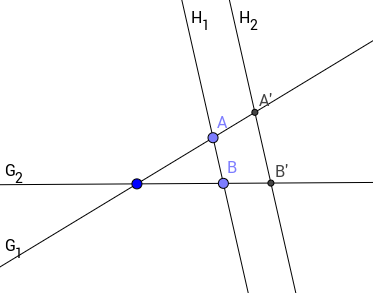
\includegraphics[height=.4\linewidth]{graphs/strahlensatz.png}
\end{figure}
\begin{align*}
\frac{\overline{ZA}}{\overline{AA'}} &= \frac{\overline{ZB}}{\overline{BB'}} \\
\frac{\overline{ZA}}{\overline{ZA'}} &= \frac{\overline{ZB}}{\overline{ZB'}} = \frac{\overline{AB}}{\overline{A'B'}} \\
\text{(Nur) Aus } \frac{\overline{ZA}}{\overline{ZA'}} &= \frac{\overline{ZB}}{\overline{ZB'}} \text{ folgt } H_1 || H_2 \\
\end{align*}

\subsection{Pythagoras}
\begin{align}
a^2+b^2 &= c^2 \Leftrightarrow \triangle ABC \text{ ist rechtwinklig} \tag{Pythagoras} \\
h^2 &= p*q \text{, wobei } h=h_c \text{ und } p,q \text{ Hypothenusenabschnitte} \tag{H\"ohensatz} \\
a^2&=cq \text{ und } b^2=cp \tag{Kathetensatz}
\end{align}

\subsection{Sinus und Kosinus}
\begin{enumerate}
\item \textbf{GAGA|HHAG}
\item
	\begin{align}
	\sin{(\varphi)} &=& -\sin{(-\varphi)} &=& \sin{(\pi - \varphi)}  &=& \sin{(\varphi + 2\pi)} &=& \cos{(\frac{\pi}{2} - \varphi)}\\
	\cos{(\varphi)} &=&  \cos{(-\varphi)} &=& -\cos{(\pi - \varphi)} &=& \cos{(\varphi + 2\pi)} &=& \sin{(\frac{\pi}{2} - \varphi)}\\
	\tan{(\varphi)} &=& -\tan{(-\varphi)} &=& \sin{(\pi + \varphi)}  & &                        &=& \tan{(\frac{\pi}{2} - \varphi)}^{-1}
	\end{align}
\item
	\begin{tabular}{c|ccccc}
	$\varphi$         & $0$ & $\frac{\pi}{6}=30^\circ$ & $\frac{\pi}{4}=45^\circ$ & $\frac{\pi}{3}=60^\circ$ & $\frac{\pi}{2}=90^\circ$ \\ \hline
	$\sin{(\varphi)}$ & $0$ & $\frac{1}{2}$            & $\frac{\sqrt{2}}{2}$     & $\frac{\sqrt{3}}{2}$     & $1$                      \\
	$\cos{(\varphi)}$ & $1$ & $\frac{\sqrt{3}}{2}$     & $\frac{\sqrt{2}}{2}$     & $\frac{1}{2}$            & $0$                      \\
	$\tan{(\varphi)}$ & $0$ & $\frac{1}{\sqrt{3}}=\frac{\sqrt{3}}{3}$   & $1$     & $\sqrt{3}$               & n.d.
	\end{tabular}
\item
	\begin{align}
	1 &= \sin{(\varphi)}^2 + \cos{(\varphi)}^2 \tag{trigonometrischer Pythagoras}\\
	\sin{(\varphi + \psi)} &= \sin{(\varphi)}\cos{(\psi)} + \cos{(\varphi)}\sin{(\psi)} \tag{Addition1}\\
	\cos{(\varphi + \psi)} &= \cos{(\varphi)}\cos{(\psi)} - \sin{(\varphi)}\sin{(\psi)} \tag{Addition2}\\
	\tan{(\varphi + \psi)} &= \frac{\tan{(\varphi)}+\tan{(\psi)}}{1-\tan{(\varphi)}\tan{(\psi)}} \tag{Addition3}\\
	\sin{(2 \varphi)} &= 2 \sin{(\varphi)}\cos{(\varphi)} \tag{Doppelwinkel1}\\
	\cos{(2 \varphi)} &= \cos{(\varphi)}^2 - \sin{(\varphi)}^2 = 1 - 2 \sin{(\varphi)}^2 = 2 \cos{(\varphi)}^2 - 1 \tag{Doppelwinkel2}\\
	\tan{(2 \varphi)} &= \frac{2\tan{(\varphi)}}{1-\tan{(\varphi)}^2} \tag{Doppelwinkel3}
	\end{align}
\item Sätze im allgemeinen Dreieck (allgemeiner Pythagoras)
	\begin{align}
	\frac{a}{\sin{\alpha}} &= \frac{b}{\sin{\beta}} = \frac{c}{\sin{\gamma}} \tag{Sinussatz}\\
	c^2 &= a^2 + b^2 - 2ab * \cos{\gamma} \tag{Cosinussatz1}\\
	a^2 &= b^2 + c^2 - 2bc * \cos{\alpha} \tag{Cosinussatz2}\\
	b^2 &= a^2 + c^2 - 2ac * \cos{\beta} \tag{Cosinussatz3}
	\end{align}
\item \[F_{\triangle ABC} = \frac{1}{2} * c * h_c = \frac{1}{2} * cb * \sin{\alpha} = \frac{1}{2} * ac * \sin{\beta} = \frac{1}{2} * ab * \sin{\gamma}\]
\item \[\sin{(\varphi)} = \frac{\tan{(\varphi)}}{\sqrt{1+\tan{(\varphi)}^2}} \text{ und } \cos{(\varphi)} = \frac{1}{\sqrt{1+\tan{(\varphi)}^2}}\]
\end{enumerate}

% TODO 7.10 rationale parametrisierung von sin/cos


\end{document}